\section{Chi-square test of independence}

%%%%%%%%%%%%%%%%%%%%%%%%%%%%%%%%%%%

\subsection{Popular kids}

%%%%%%%%%%%%%%%%%%%%%%%%%%%%%%%%%%%

\begin{frame}
\frametitle{Popular kids}

\dq{In the dataset \texttt{popular}, students in grades 4-6 were asked whether good grades, athletic ability, or popularity was most important to them. A two-way table separating the students by grade and by choice of most important factor is shown below. Do these data provide evidence to suggest that goals vary by grade?}

\twocol{0.5}{0.5}
{
\begin{center}
\begin{tabular}{rrrr}
  \hline
 & Grades & Popular & Sports \\ 
  \hline
$4^{th}$ &  63 &  31 &  25 \\ 
$5^{th}$ &  88 &  55 &  33 \\ 
$6^{th}$ &  96 &  55 &  32 \\ 
   \hline
\end{tabular}
\end{center}
}
{
\begin{center}
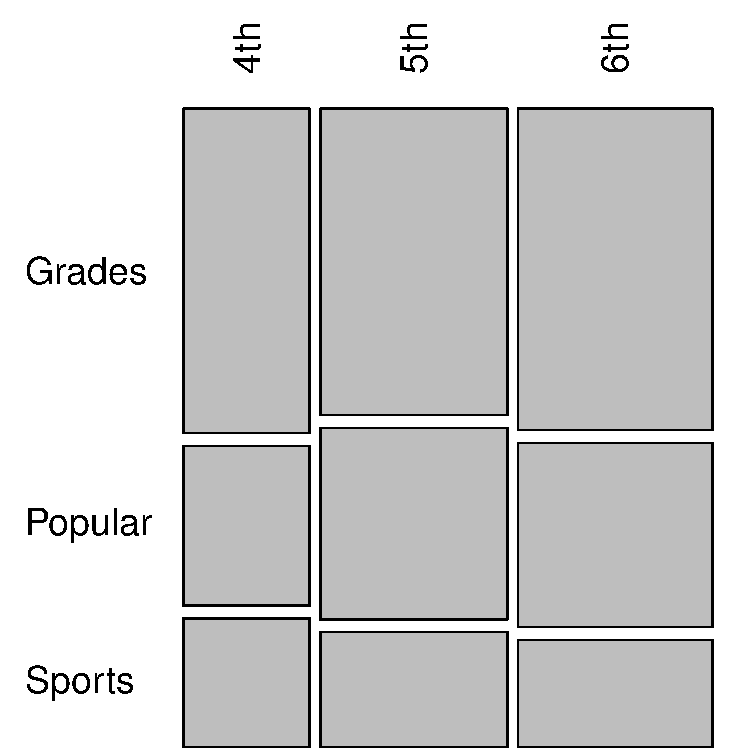
\includegraphics[width=0.8\textwidth]{6-4_chisq_indep/figures/popular/popular_mosaic}
\end{center}
}


\end{frame}

%%%%%%%%%%%%%%%%%%%%%%%%%%%%%%%%%%%

\begin{frame}
\frametitle{Chi-square test of independence}

\begin{itemize}
\item The hypotheses are:
\begin{itemize}
\item[$H_0$:] Grade and goals are independent. Goals do not vary by grade.
\item[$H_A$:] Grade and goals are dependent. Goals vary by grade.
\end{itemize}

\pause

\item The test statistic is calculated as
\[ \chi^2_{df} = \sum_{i = 1}^{k} \frac{(O - E)^2}{E} \quad \text{ where } \quad df = (R - 1) \times (C - 1), \]
where $k$ is the number of cells, $R$ is the number of rows, and $C$ is the number of columns.

\Note{We calculate $df$ differently for one-way and two-way tables.}

\pause

\item The p-value is the area under the $\chi^2_{df}$ curve, above the calculated test statistic.

\end{itemize}


\end{frame}

%%%%%%%%%%%%%%%%%%%%%%%%%%%%%%%%%%%

\subsection{Expected counts in two-way tables}

%%%%%%%%%%%%%%%%%%%%%%%%%%%%%%%%%%%

\begin{frame}
\frametitle{Expected counts in two-way tables}

\formula{Expected counts in two-way tables}
{
\[ \text{Expected Count} = \frac{(\text{row total}) \times (\text{column total})}{\text{table total}} \]
}

\pause

{\small
\begin{center}
\begin{tabular}{rrrr|r}
  \hline
 & Grades & Popular & Sports	& Total \\ 
  \hline
$4^{th}$ &  \orange{63} &  \green{31} &  25 	&119 \\ 
$5^{th}$ &  88 &  55 &  33	& 176 \\ 
$6^{th}$&  96 &  55 &  32	& 183 \\ 
   \hline
Total	& 247	& 141	& 90	& 478 \\
\end{tabular}
\end{center}
}

\pause

\[ \orange{$E_{row~1, col~1} = \frac{119 \times 247}{478} = 61$} \qquad \pause
 \green{$E_{row~1, col~2} = \frac{119 \times 141}{478} = 35$} \]

\end{frame}

%%%%%%%%%%%%%%%%%%%%%%%%%%%%%%%%%%%

\begin{frame}
\frametitle{Expected counts in two-way tables}

\pq{What is the expected count for the highlighted cell?}

{\small
\begin{center}
\begin{tabular}{rrrr|r}
  \hline
 & Grades & Popular & Sports	& Total \\ 
  \hline
$4^{th}$ &  63 &  31 &  25 	&119 \\ 
$5^{th}$ &  88 &  \red{55} &  33	& 176 \\ 
$6^{th}$ &  96 &  55 &  32	& 183 \\ 
   \hline
Total	& 247	& 141	& 90	& 478 \\
\end{tabular}
\end{center}
}

\twocol{0.2}{0.8}
{
\begin{enumerate}[(a)]
\solnMult{$\frac{176 \times 141}{478}$}
\item $\frac{119 \times 141}{478}$
\item $\frac{176 \times 247}{478}$
\item $\frac{176 \times 478}{478}$
\end{enumerate}
}
{
\soln{\only<2>{
\red{$\rightarrow$ 52\\
{\small more than expected \# of 5th graders \\
have a goal of being popular}}
\vspace{0.75cm}
}
}
}

\end{frame}

%%%%%%%%%%%%%%%%%%%%%%%%%%%%%%%%%%%

\begin{frame}
\frametitle{Calculating the test statistic in two-way tables}

Expected counts are shown in \ex{blue} next to the observed counts.
\begin{center}
\begin{tabular}{rrrr|r}
  \hline
 & Grades & Popular & Sports	& Total \\ 
  \hline
$4^{th}$ 	&  63 \ex{61} &  31 \ex{35} &  25 \ex{23}	&119 \\ 
$5^{th}$ 	&  88 \ex{91} &  55 \ex{52} &  33 \ex{33}	& 176 \\ 
$6^{th}$	&  96 \ex{95} &  55 \ex{54} &  32 \ex{34}	& 183 \\ 
   \hline
Total	& 247	& 141	& 90	& 478 \\
\end{tabular}
\end{center}

\vspace{0.5cm}

\pause

\begin{eqnarray*} 
\chi^2 &=& \sum \frac{(63 - 61)^2}{61} + \frac{(31 - 35)^2}{35} + \cdots + \frac{(32 - 34)^2}{34} = 1.3121 \\
\pause
df &=& (R - 1) \times (C - 1) = (3 - 1) \times (3 - 1) = 2 \times 2 = 4 
\end{eqnarray*}

\end{frame}

%%%%%%%%%%%%%%%%%%%%%%%%%%%%%%%%%%%

\subsection{Results}

%%%%%%%%%%%%%%%%%%%%%%%%%%%%%%%%%%%

\begin{frame}
\frametitle{Calculating the p-value}

\pq{Which of the following is the correct p-value for this hypothesis test?
\[ \chi^2 = 1.3121 \qquad df = 4 \]
}

\twocol{0.6}{0.4}{
\begin{center}
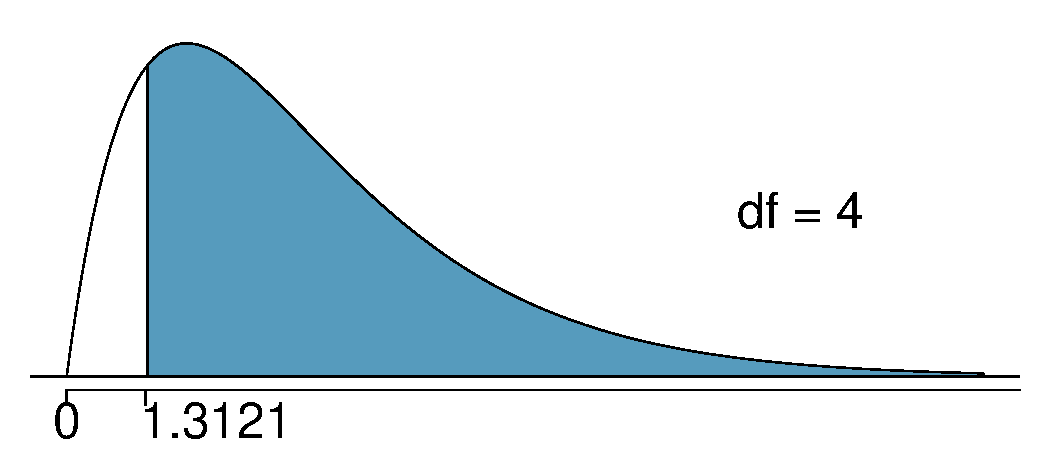
\includegraphics[width=0.67\textwidth]{6-4_chisq_indep/figures/popular/popular}
\end{center}
}
{
{\small
\begin{enumerate}[(a)]
\setlength{\itemsep}{0in}
\solnMult{ more than 0.3}
\item between 0.3 and 0.2
\item between 0.2 and 0.1
\item between 0.1 and 0.05
\item less than 0.001
\end{enumerate}
}
}

\begin{center}
{\scriptsize
\begin{tabular}{r | rrrr | rrrr |}
  \hline
Upper tail & 0.3 & 0.2 & 0.1 & 0.05 & 0.02 & 0.01 & 0.005 & 0.001 \\ 
  \hline
df \hfill 1 &  1.07 &  1.64 &  2.71 &  3.84 &  5.41 &  6.63 &  7.88 &  10.83 \\ 
  2 &  2.41 &  3.22 &  4.61 &  5.99 &  7.82 &  9.21 &  10.60 &  13.82 \\ 
  3 &  3.66 &  4.64 &  6.25 &  7.81 &  9.84 &  11.34 &  12.84 &  16.27 \\ 
  4 &  4.88 &  5.99 &  7.78 &  9.49 &  11.67 &  13.28 &  14.86 &  18.47 \\ 
  5 &  6.06 &  7.29 &  9.24 &  11.07 &  13.39 &  15.09 &  16.75 &  20.52 \\ 
\end{tabular}
}
\end{center}

\end{frame}

%%%%%%%%%%%%%%%%%%%%%%%%%%%%%%%%%%%

\begin{frame}
\frametitle{Conclusion}

\dq{Do these data provide evidence to suggest that goals vary by grade?}

\begin{itemize}

\item[$H_0$:] Grade and goals are independent. Goals do not vary by grade.

\item[$H_A$:] Grade and goals are dependent. Goals vary by grade. \\

\end{itemize}

$\:$ \\

\soln{\only<2>{Since p-value is high, we fail to reject $H_0$. The data do not provide convincing evidence that grade and goals are dependent. It doesn't appear that goals vary by grade.
}
}

\end{frame}
